\apendice{Plan de Proyecto Software}


\section{Introducción}

En este apartado se recoge el ciclo de vida del proyecto, detallando los aspectos más relevantes del mismo y como se han resuelto los diferentes problemas a lo largo de su desarrollo. Se presentarán secciones que muestran de manera cronológica la justificación de las decisiones tomadas.

Para llevar a cabo este seguimiento y planificación del proyecto se ha utilizado una metodología Scrum, que ha permitido un desarrollo ágil dividido en \textit{sprints} de dos semanas cada uno. 
Al comienzo de cada \textit{sprint} se establecen las tareas y objetivos a realizar durante ese periodo. Al final de cada \textit{sprint} se realizan reuniones con los tutores para valorar los resultados obtenidos y definir nuevas tareas para el siguiente \textit{sprint}.
Para organizar las diferentes tareas se ha usado Gitlab que permite visualizar los diferentes estados de desarrollo de las tareas.


\section{Planificación temporal}

La propuesta del proyecto consistía en crear una aplicación Android basada en \textit{blockchain} que simplifica la contratación y la verificación a través de contratos inteligentes.
Los requisitos principales del proyecto se pueden dividir en los siguiente puntos:

\begin{itemize}

\item \textbf{Tecnología \textit{blockchain}:} Utilizar la tecnología \textit{blockchain} para desplegar contratos inteligentes que gestionen automáticamente los contratos laborales, desde su creación hasta su ejecución.

\item \textbf{Contratos Inteligentes:} Implementar contratos inteligentes en Solidity.


\item \textbf{Identificación segura mediante dispositivo móvil:} Implementar autenticación biométrica y el escaneo de códigos QR.

\item \textbf{Integración con Pagos:} Incorporar procesamiento de pagos dentro de la aplicación para facilitar transacciones rápidas y seguras

\item \textbf{Desarrollo de Aplicación Móvil:} Diseñar una interfaz de usuario amigable para dispositivos móviles que facilite la creación de contratos, seguimiento y pago.

\end{itemize}

Una vez expuestos los requerimientos principales del proyecto, la etapa inicial del proyecto se basó en una exhaustiva investigación, que permitió obtener un conocimiento detallado sobre las tecnologías y herramientas necesarias. Dado que inicialmente no contaba con conocimientos previos en desarrollo de aplicaciones móviles y tecnología \textit{blockchain}, esta investigación fue crucial para identificar las mejores prácticas y soluciones en estos campos. 
Esta etapa de investigación y adaptación a las nuevas tecnologías tuvo una duración de aproximadamente 3 semanas, durante las cuales se hizo especial énfasis en entender a fondo el funcionamiento de la blockchain y los contratos inteligentes.
Este aprendizaje teórico se reforzó de manera práctica con diversos proyectos usando Truffle, completando videotutoriales y realizando el curso interactivo `CryptoZombies', además de consultar numerosos artículos especializados. Estas actividades facilitaron la asimilación del nuevo lenguaje de programación y familiarización con el entorno \textit{blockchain}.


\subsubsection{Sprint 0}

Este \textit{sprint} se desarrolló entre los días 3 y 17 de noviembre de 2023. Se realizaron las siguientes tareas y objetivos:

\begin{enumerate}

\item \textbf{Configuración repositorio:} Se configuró el repositorio en GitLab y se establecieron ramas principales basadas en el flujo de trabajo de GitFlow, incluyendo 'main' para la producción y 'develop' para el desarrollo 

\item \textbf{Configuración entorno para la redacción de la memoria:} Se descargaron las plantillas y se configuró el software de redacción "Texmaker".

\item \textbf{Investigación de tecnologías para realizar una app móvil:} Se realizó un análisis comparativo de las plataformas de desarrollo móvil más populares. Se evaluaron criterios como el rendimiento, la facilidad de uso y la comunidad de desarrolladores.

\item \textbf{Diseñar la arquitectura del proyecto:} Se definieron los componentes principales del sistema y su interacción. Para facilitar la compresión de la estructura y el flujo de datos se desarrollaron diagramas.

\end{enumerate}


\subsubsection{Sprint 1}

Este \textit{sprint} se desarrolló entre los días 17 de noviembre y 1 de diciembre de 2023. Se realizaron las siguientes tareas y objetivos:

\begin{enumerate}

\item \textbf{Investigación \textit{smart contracts}:} Se evaluó la elección entre usar \textit{tokens} fungibles o no fungibles para el desarrollo de los contratos, optándose finalmente por el estándar ERC-721, característico de los NFTs, debido a su adaptabilidad al proyecto.
A partir de esta decisión fue necesario evaluar la versión adecuada para el compilador de solidity que asegure la compatibilidad con ciertas bibliotecas necesarias.

\item \textbf{Creación de un prototipo visual:} Se diseñó un prototipo visual inicial para la aplicación móvil utilizando herramientas como Figma y Canva.
El prototipo se centró en crear una interfaz intuitiva y atractiva que refleje las funcionalidades claves del proyecto.

\end{enumerate}


\subsubsection{Sprint 2}

Este \textit{sprint} se desarrolló entre los días 1 de diciembre y 21 de diciembre de 2023. Se realizaron las siguientes tareas y objetivos:

\begin{enumerate}

\item \textbf{Primera implementación del contrato inteligente:} Siguiendo el estándar ERC-721 se planteó una primera solución que incluyese las funcionalides básicas de creación y transferencia de NFTs de manera segura y eficiente.

\item \textbf{Configuración entorno de desarrollo aplicación móvil:} Se configuró el entorno de desarrollo para asegurar la correcta conectividad entre la aplicación móvil y el \textit{backend}, representado por el \textit{blockchain} y el contrato inteligente.


\end{enumerate}


\subsubsection{Sprint 3}

Este \textit{sprint} se desarrolló entre los días 21 de diciembre de 2023 y 12 de enero de 2024. Se realizaron las siguientes tareas y objetivos:

\begin{enumerate}

\item \textbf{Continuación con la implementación del contrato inteligente:} Se continuó con el desarrollo del contrato inteligente implementando funciones que manejasen la lógica de los pagos dentro de la app. También se programó la lógica para la correcta destrucción del contrato una vez ha transcurrido su ciclo de vida.

\item \textbf{Creación de pruebas unitarias para comprobar el correcto funcionamiento del contrato inteligente:}  Para garantizar el correcto funcionamiento del contrato inteligente se realizaron test en Java utilizando las herramientas Ganache y Truffle.
Ganache sirvió para simular un entorno \textit{blockchain} local y Truffle sirvió para compilar, migrar y probar el contrato inteligente con los test creados.

\item \textbf{Implementar navegación en la aplicación móvil:} Se programaron las pantallas principales de la aplicación. Estas pantallas se integraron mediante un menú interactivo que facilita la navegación dentro de la app mejorando la experiencia del usuario.

\item \textbf{Tareas de ordenación de repositorio:} Se realizaron taras de ordenación y limpieza en el repositorio del código. Incluyó la reorganización de directorios, la eliminación de archivos obsoletos y la estandarización de nombres de archivos y carpetas para mejorar la accesibilidad y el mantenimiento.

\item \textbf{Modificación del ReadMe:} Se actualizó el archivo ReadMe para reflejar los cambios recientes en el proyecto y proporcionar una guía más clara y detallada para los usuarios que quieran replicar el proyecto.

\end{enumerate}

Debido a las fechas de vacaciones de Navidad, a los compromisos académicos y la gran demanda de los \textit{issues}, no se logró completar lo previsto para este \textit{sprint}, por lo que se decidió en la reunión del 12 de Enero ampliar 2 semanas más este \textit{sprint}.


\subsubsection{Sprint 4}

Este \textit{sprint} se desarrolló entre los días 26 de enero y 9 de febrero de 2024. Se realizaron las siguientes tareas y objetivos:

\begin{enumerate}

\item \textbf{Integración de Metamask:} Se integró la billetera Metamask para facilitar las transacciones en la aplicación. Esto incluyó configurar la autenticación y las firmas de transacciones a través de la popular billetera de criptomonedas, permitiendo a los usuarios interactuar de manera segura a través de la extensión de navegador de Metamask.

\item \textbf{Documentación de tecnologías utilizadas:}  Tras el progresivo avance del proyecto y el amplio repertorio de \textit{frameworks} y librerías utilizadas, se plasmaron y explicaron todas ellas en su correspondiente apartado en la memoria.

\end{enumerate}


\subsubsection{Sprint 5}

Este \textit{sprint} se desarrolló entre los días 9 de febrero y 23 de febrero de 2024. Se realizaron las siguientes tareas y objetivos:

\begin{enumerate}

\item \textbf{Creación de la guía de instalación:} Se elaboró una guía de instalación detallada para facilitar la configuración inicial del sistema por parte de los usuarios. Recogiendo las instrucciones paso a paso para la instalación del software, configuración del entorno y la conexión con las dependencias necesarias.

\item \textbf{Documentación del contexto teórico:}  Se empezó a recoger en la memoria todos los fundamentos teóricos que fundamentan este proyecto, proporcionando una base sólida que ayude a entender el marco en el que se desarrolla la aplicación. 

\item \textbf{Implementación de pantallas informativas:} Se implementaron dos pantallas clave en la aplicación móvil: la pantalla `Wallet', que permite al usuario la conexión con la billetera y muestra los datos de la cuenta seleccionada en la billetera Metamask, y la pantalla `Info', que incluye información actualizada sobre el precio del Ethereum, junto con un gráfico interactivo y una calculadora para conversiones.

\item \textbf{Implementar funcionalidad modificar contrato:} Se extendieron las funciones del contrato inteligente para permitir modificar un contrato existente. Esto incluyó la adición de métodos para actualizar parámetros del contrato y funciones que permiten a los usuarios adaptar el contrato a necesidades cambiantes, asegurando así una mayor flexibilidad.

\item \textbf{Creación base de datos para el almacenamiento de las cuentas de los usuario:}  Se implementó una base de datos utilizando Firebase de Google, aprovechando la amplia gama de funcionalidades que incluye. De esta forma se permitía a los usuarios iniciar sesión con su cuenta google, Facebook y Github entre muchas otras, facilitando un proceso de autenticación rápido y seguro, además de almacenar de manera eficiente los datos de las cuentas de los usuarios.

\end{enumerate}


\subsubsection{Sprint 6}

Este \textit{sprint} se desarrolló entre los días 23 de febrero y 8 de marzo de 2024. Se realizaron las siguientes tareas y objetivos:

\begin{enumerate}

\item \textbf{Modularizar código:} Debido a que los \textit{smart contracts} en la Ethereum Virtual Machine (EVM) están sujetos a una restricción de tamaño para prevenir ataques de denegación de servicio, el contrato que me encontraba desarrollando se encontraba en el límite de tamaño permitido, impidiendo futuras ampliaciones. 
Para resolver esto, se optó por modularizar el contrato inteligente en diferentes componentes. Esto no solo evitó la necesidad de desplegar múltiples contratos, lo cual hubiera sido más costoso en términos de gas, sino que también ayudó en la organización del código.

\item \textbf{Validación de datos de entrada en \textit{smart contracts}:} Aunque inicialmente el contrato inteligente ya incluía algunas comprobaciones básicas en el código Solidity y la aplicación también verificaba las entradas, se realizaron mejoras significativas en estas validaciones para reforzar la seguridad.

\item \textbf{Ampliación funcionalidad SmartContract:} Se añadió código adicional al contrato inteligente para permitir que usuarios adicionales, aparte del dueño original, pudieran tener permisos de gestión del contrato. Esto fue diseñado para facilitar la colaboración permitiendo que usuarios autorizados puedan realizar cambios sin depender el propietario inicial.

\item \textbf{Modificación lógica contrato:} Se modificó la lógica del contrato para permitir la creación de contratos sin asignar inicialmente un trabajador. Esta funcionalidad permitió mostrar contratos disponibles en una especie de "tablón de ofertas de trabajo", donde las personas en búsqueda de empleo pueden encontrar y seleccionar contratos que coincidan con sus habilidades y expectativas.

\end{enumerate}

Los siguientes objetivos que se exponen a continuación, no han podido ser completados y han sido pospuestos hasta el \textit{sprint} 10.
Hasta ahora, la aplicación se ha estado probando de manera local en una pestaña del navegador por razones de eficiencia y comodidad. Sin embargo, al intentar realizar las pruebas con un teléfono móvil para funcionalidades que requieren ejecución nativa, como el escaneo de códigos QR o el acceso a la ubicación, se han encontrado errores debido a incompatibilidades con las bibliotecas y el sistema operativo Android.  
Por tanto, estos problemas se han tenido que posponer hasta que se solucione el problema de compatibilidad de la app con la biblioteca web3.

\begin{enumerate}

\item \textbf{Implementación de códigos QR:} La integración de códigos QR, diseñada para facilitar transacciones rápidas y seguras mediante escaneo, se ha pospuesto debido a problemas técnicos encontrados durante las pruebas en dispositivos móviles.

\item \textbf{Inclusión ubicación a los parámetros del contrato:} Del mismo modo que con los códigos QR, por la imposibilidad de probar los servicios de ubicación en un dispositivo móvil, se ha tenido que posponer.

\item \textbf{Creación de un filtro para buscar contratos:}  Este \textit{issue} ha sido pospuesto ya que depende directamente de la incorporación de la ubicación como parámetro para realizar el filtro.

\item \textbf{Creación de eventos para registrar alertas en los contratos:} Debido a la importancia de solucionar el problema de despliegue en teléfonos móvil, este \textit{issue} ha pasado a segundo plano.

\end{enumerate}


\subsubsection{Sprint 7}

Este \textit{sprint} se desarrolló entre los días 8 de marzo y 22 de marzo de 2024. Se realizaron las siguientes tareas y objetivos:

\begin{enumerate}

\item \textbf{Resolver error compatibilidad app android y biblioteca web3:} Este \textit{issue} tuvo prioridad máxima dentro del \textit{sprint}. Al ejecutar la aplicación en un dispositivo móvil aparecía un problema de compatibilidad significativo entre la biblioteca web3 y el motor JavaScript Hermes utilizado en React Native.
Este problema incapacita cualquier avance para el que se requiriese las funcionales nativas del dispositivo móvil.

\item \textbf{Adaptar aplicación web a aplicación móvil:} La aplicación en su primera etapa de desarrollo fue hecha desde un entorno web. Por lo que una vez solucionado el problema anterior que impedía desplegar el proyecto en un dispositivo móvil, fue necesario enfrentarse a diversos desafíos adicionales al adaptar características específicas de la web para funcionar en un entorno móvil.

\end{enumerate}

Después de varias horas de esfuerzo, se logró identificar y corregir el error más importante hasta el momento. Además de cumplir con los requisitos establecidos para este \textit{sprint}, también se consiguió implementar la funcionalidad para mostrar códigos QR con los detalles del contrato, el cual era uno de los objetivos que habían quedado pendientes del \textit{sprint} anterior. 

\subsubsection{Sprint 8}

Este \textit{sprint} se desarrolló entre los días 22 de marzo y 5 de abril de 2024. Se centró principalmente en resolver desafíos relacionados con la migración de la aplicación web a móvil, especialmente en lo que respecta a la conectividad con la billetera externa Metamask.

Se realizaron las siguientes tareas y objetivos:

\begin{enumerate}

\item \textbf{Importar cuentas de Ganache a la app móvil de Metamask:} Esto representaba inicialmente una fase intermedia entre las pruebas locales y el despliegue en una red real.
Por errores de conexión se llego a la conclusión de que no era posible, por lo que se decidió omitir este paso ya que su eliminación no afecta el progreso hacia el entorno de producción.

\item \textbf{Gestionar conexión de la billetera desde la app:} Directamente conectar con Metamask resultó inviable debido a restricciones técnicas, por lo que se evaluó para adaptar el sistema para utilizar WalletConnect junto con las librerías Wagmi y Viem, permitiendo la conexión con más de 300 billeteras diferentes

\end{enumerate}

\subsubsection{Sprint 9}

El \textit{sprint} 9 tuvo lugar del 5 al 19 de abril. Durante estas dos semanas, me centré intensamente en adaptar la aplicación para su uso en un contexto global.

El objetivo principal de este \textit{sprint} fue adaptar la aplicación a un entorno de producción, cambiando toda la codificación de la biblioteca web3 a la biblioteca ethers. Este cambio requería no sólo reemplazar las librerías, sino también asegurarse de que todas las funcionalidades existentes fueran compatibles y operativas con ethers.
Además, tras la implementación de WalletConnect en la aplicación hizo necesario adaptar todas las funcionalidades que interactuasen con la \textit{blockchain} al funcionamiento de WalletConnect.
Paralelamente a las modificaciones técnicas, se estableció un objetivo adicional de documentar los nuevos avances realizados en el proyecto hasta la fecha. 

Aunque el sprint estuvo marcado por un único objetivo técnico, la amplitud de este trabajo fue considerable. Abarcó todo el período del \textit{sprint}.


\subsubsection{Sprint 10}

El \textit{sprint} 10 tuvo lugar del 19 de abril al 3 de mayo. Al igual que en el \textit{sprint} anterior, este lapso de tiempo viene marcado por un único objetivo.

Con la aplicación en una etapa avanzado de desarrollo, se identificó la necesidad de acreditar al usuario con datos personales en la aplicación. Hasta ahora, los usuarios se identificaban únicamente mediante la dirección de su billetera, lo que les proporcionaba anonimato. Sin embargo, para evitar este estado de anonimato, identificamos la necesidad de asociar a cada usuario con datos personales que permitan su validación legal.
El trabajo en este \textit{sprint} fue identificar qué datos personales son necesarios para acreditar al usuario y cómo se podrían manejar en mi aplicación.
Finalmente se decidió implementar una pestaña perfil donde se recojan todos estos datos, aparte de la funcionalidad de que el usuario pueda actualizarlos.


\subsubsection{Sprint 11}

Este \textit{sprint} se desarrolló entre el 3 y 17 de mayo y se centró en resolver problemas de compatibilidad y preparar la aplicación para un rendimiento óptimo. 
Los objetivos principales son los siguientes:

\begin{enumerate}

\item \textbf{Preparación de la aplicación para funcionamiento total con Ganache}: Debido a los númerosos desafíos de lanzar la aplicación a un ámbito global, se llegó la decisión de descartar el uso de WalletConnect y su inclusión en la \textit{blockchain} real. Esto implicó revertir el desarrollo aproximadamente mes y medio para asegurar que la aplicación funcionara de manera integral con Ganache, lo que permitió una simulación eficaz del entorno \textit{blockchain} en desarrollo y pruebas.

\item \textbf{Resolución de incompatibilidades con Expo}: Durante la adaptación de la aplicación a su uso con Ganache, surgieron problemas al desplegar la aplicación. Estos fueron resueltos de manera eficiente actualizando Expo a su última versión, lo que permitió su despliegue.

\item \textbf{Investigación sobre la viabilidad de implementación de base de datos con Ganache}: Se planteó la idea de integrar la dirección de la billetera Ganache en el perfil del usuario almacenado en la base de datos, permitiendo su recuperación directa. Optimizando la gestión de los datos dentro de la aplicación.

\item \textbf{Arreglo de Incompatibilidad entre Firebase y Web3}: Se detectó y resolvió una incompatibilidad crítica entre la autenticación de Firebase y el uso de la biblioteca Web3. 
El problema se solucionó implementando una importación perezosa de Web3, que se activa solo después de una autenticación exitosa con Firebase, esquivando así el error producido por la incompatibilidad de ambas bibliotecas.

\end{enumerate}

Con el final del \textit{sprint} 11 el 17 de mayo de 2024, se concluye el ciclo de desarrollo activo de la aplicación. El tiempo restante hasta la presentación del proyecto se ha dedicado a revisar el código, finalizar los últimos detalles en la memoria del proyecto, y asegurarnos de que todos los componentes funcionen correctamente en conjunto.

En la imagen \ref{fig:GanttScrum} se puede visualizar el cronograma completo de las tareas del proyecto, mostrando la duración y secuencia de cada tarea programada a lo largo de los diversos \textit{sprints}, facilitando la comprensión de las fases de desarrollo.

\begin{landscape}
\begin{figure}[h]
	\caption[Diagrama Gantt sprints]{Diagrama Gantt que muestra la cronología temporal de los \textit{sprints}}
	\centering
	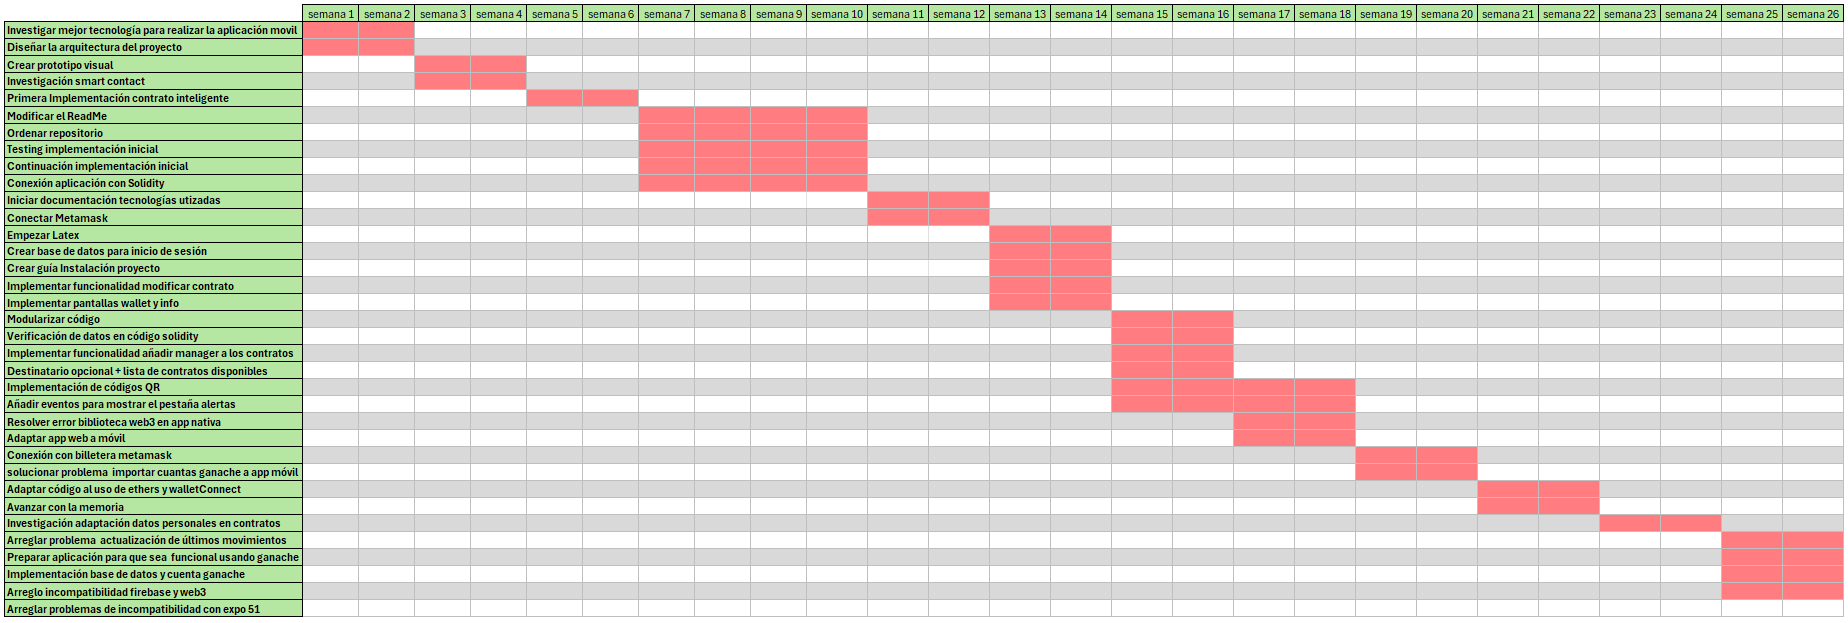
\includegraphics[scale=0.5]{GanttScrum}
	\label{fig:GanttScrum}
\end{figure}
\end{landscape}


\section{Estudio de viabilidad}

El estudio de viabilidad es un análisis crítico realizado para evaluar la posibilidad y conveniencia de llevar a cabo un proyecto específico.
Para determinar si este proyecto es viable, se van a desarrollar la viabilidad económica y la viabilidad legal.

\subsection{Viabilidad económica}

La viabilidad económica de un proyecto evalúa si los beneficios económicos previstos justifican los costos involucrados.
Se considerarán los costes de recursos humanos, el material empleado y el software usado.

\subsubsection{Coste de personal}

Para realizar una estimación de los costos del proyecto, vamos a acotar el cálculo a una duración de 9 meses, que ha sido el tiempo empleado en realizar el proyecto.
Por otro lado, como solo ha habido una persona desarrollando el proyecto (el alumno), se va a considerar un único trabajador para los cálculos.
Partiendo de un salario base promedio de un programador junior en España de 21000 brutos anuales, podemos estimar que el coste total personal sería el expuesto en la tabla \ref{tab:costoPersonal}.

\begin{table}[p]
	\centering
	\begin{tabular}{l r}
		\toprule
		\textbf{Concepto} &  \textbf{Coste} \\
		\midrule
		Salario bruto (anual) & 21000 \\
		Retención del IRPF (12\%) & 2520  \\
		Seguridad Social (28,3\%) & 5943 \\
		Salario neto (anual) & 12537 \\
		Salario neto (mensual) & 1044,75 \\
		\midrule
		\textbf{Coste total en los 9 meses} & 15750 \\
		\bottomrule
	\end{tabular}
	\caption{Coste total del personal}
	\label{tab:costoPersonal}
\end{table}



\subsubsection{Coste hardware}

En cuanto al coste del \textit{hardware} para la realización del proyecto únicamente ha sido necesario contar con un ordenador para el desarrollador.
El ordenador utilizado para el desarrollo tiene una antigüedad de 7 años, por lo que ya ha sido amortizado y se desprecia su coste.

\subsubsection{Coste software}

Las herramientas de software empleadas en este proyecto son principalmente gratuitas; sin embargo, los servicios de Firebase e Infura presentan ciertas restricciones en sus versiones sin costo que podrían limitar la operatividad al escalar la aplicación.
Firabase en su versión gratuita ofrece 1 GiB de almacenamiento, que es un limitante, y soporta hasta 50000 usuarios activos mensuales.
Por otro lado, Infura proporciona 100000 peticiones diarias gratuitamente.

Considerando un escenario de total éxito en el lanzamiento de la aplicación, donde se estimen unos 200000 usuarios activos mensuales, las necesidades podrían requerir una gran ampliación de almacenamiento, lo cual vendría acompañado de un gran volumen de operaciones sobre la base de datos.
Para Infura se contemplaría la necesidad de escalar al plan más avanzado, que permite hasta 5 millones de peticiones diarias.

Los costos, inicialmente en dólares han sido convertidos a euros a 0,92€. Ver tabla \ref{tab:costeSoftware}.

\begin{table}[p]
	\centering
	\begin{tabular}{l r}
		\toprule
		\textbf{Concepto} &  \textbf{Coste} \\
		\midrule
		    Infura & 917,90 \\
    190500000 operaciones lectura & 113 \\
    999 GiB Almacenamiento & 165,22 \\
    53100000 operaciones escritura & 86,74 \\
    200000 usuarios activos & 633,35 \\
		\midrule
		\textbf{Coste total mensual} & 1916,21 \\
		\bottomrule
	\end{tabular}
	\caption{Coste total del Software}
	\label{tab:costeSoftware}
\end{table}


A este resultado queda sumar el coste de lanzar la aplicación al mercado, el cual viene dado por una tasa que aplica Google al subir la aplicación a la Play Store. Por lo que sería sumar al coste total un pago único de 25 dolares (23,36 euros).

\subsubsection{Beneficios}

El proyecto no se ha realizado con el objetivo de obtener un beneficio económico. Este producto ha sido desarrollado con el fin de implementar una herramienta para abordar los desafíos del mercado laboral, especialmente en sectores afectados por la informalidad como la agricultura y los servicios domésticos.
Se considera por tanto, que este proyecto tiene un carácter social, destinado a mejorar las condiciones laborales y a promover la equidad en el trabajo. 

Se considera que la financiación del proyecto debería provenir principalmente de inversores interesados en la optimización y reducción de costes del proceso de contratación.
Adicionalmente, el gobierno español representa un potencial inversor clave, ya que podría promover activamente el uso de esta aplicación para fomentar prácticas laborales adecuadas y combatir la economía sumergida. 


\subsection{Viabilidad legal}

Esta sección se centra en analizar los aspectos legales asociados con el desarrollo y distribución de una solución basada en \textit{blockchain}.
Los puntos claves que incluyen el análisis de las licencias de software y el cumplimiento de las leyes vigentes.

\subsection{Licencias de software}

En el proyecto se emplea diversas bibliotecas y frameworks que están regidos bajo licencias de software específicas (ver tabla \ref{tab:licenciasSoftware}), que definen los términos y condiciones para su uso, modificación y distribución.
A continuación, se va a listar las diferentes licencias de cada dependencia de mi proyecto, en orden de menos restrictiva a más restrictiva:

\begin{itemize}

\item \textbf{Licencia MIT:} No impone restricciones significativas, permitiendo uso comercial, modificación, distribución y uso privado.

\item \textbf{Licencia Apache 2.0:} Similar a la licencia MIT, pero también proporciona una protección explícita contra patentes.

\item \textbf{Términos de servicio de Google:} Específicos para los productos de Google, no son licencias de software como tal, pero regulan cómo se pueden usar los servicios.

\item \textbf{GNU GPL:} Permite uso comercial, modificación, distribución y uso privado, pero cualquier versión modificada debe también ser libre.

\item \textbf{GNU GPL-3.0:} Similar a la GPL pero con términos adicionales para cerrar algunas brechas legales en ciertos escenarios.

\end{itemize}


\begin{table}[p]
	\centering
	\begin{tabular}{l r}
		\toprule
		\textbf{Dependencia} &  \textbf{Licencia} \\
		\midrule
    React Native & Licencia MIT \\
    Expo & Licencia MIT \\
    Firebase & Términos de servicio de Google \\
    Solidity & Licencia GPL-3.0 \\
    Remix & Licencia GPL-3.0 \\
    Truffle & Licencia MIT \\
    Ganache & Licencia MIT \\
    MetaMask & Licencia GPL-3.0 \\
    WalletConnect & Licencia MIT \\
    Node.js & Licencia MIT \\
    OpenZeppelin & Licencia Apache 2.0 \\
    web3 & Licencia MIT \\
    ethers & Licencia MIT \\
		\midrule
		\textbf{Coste total mensual} & 1916,21 \\
		\bottomrule
	\end{tabular}
	\caption[Licencias proyecto]{Dependencias del proyecto y licencias bajo las cuales están registradas}
	\label{tab:licenciasSoftware}
\end{table}


\subsection{Regulación legal}

Debido a que este proyecto implicará la gestión de datos personales, es fundamental cumplir con el Reglamento General de Protección de Datos (RGPD) de la UE y la legislación española correspondiente, como la Ley Orgánica de Protección de Datos Personales y garantía de los derechos digitales (LOPDGDD). Esto implica garantizar la protección adecuada de los datos personales y obtener consentimientos claros por parte de los usuarios para usar sus datos.

Actualmente no hay ninguna legislación vigente en España en cuanto a los contratos inteligentes. Sin embargo, estos deberían de cumplir con el código civil en términos de formación de contratos, capacidad para contratar y consentimiento.
Por supuesto, la aplicación deberá cumplir con la legislación laboral española, asegurando que los contratos creados cumplan con las normativas de trabajo, incluyendo las mínimas garantías y derechos para los trabajadores.
